\documentclass[11pt,a4paper]{scrartcl}
\typearea{12}
\usepackage{graphicx}
\usepackage{pstricks}
\usepackage{listings}

\usepackage{tikz}
\usepackage{tikzscale}
\usepackage{pgfplots}

\usepackage{pgf}
\usepackage[utf8]{inputenc}
\usetikzlibrary{arrows,automata}
\usetikzlibrary{positioning}


\tikzset{
    neuron/.style={
           rectangle,
           rounded corners,
           draw=black, very thick,
           inner sep=2pt,
           text centered,
           },
}


\tikzset{
    gc/.style={
           rectangle,
           rounded corners,
           draw=red, very thick,
           inner sep=2pt,
           text centered,
           },
}


\tikzset{
    io/.style={
           rectangle,
           rounded corners,
           draw=green, very thick,
           inner sep=2pt,
           text centered,
           },
}


\tikzset{
    on/.style={
           circle,
           draw=red, very thick,
           inner sep=4pt,
           fill=red!45,
           },
}


\tikzset{
    off/.style={
           circle,
           draw=blue, very thick,
           inner sep=4pt,
           text centered,
           },
}



\pgfplotsset{compat=1.8}


\lstset{language=python}
\pagestyle{headings}
\markright{Computational Neuroscience - Lecture 21}
\begin{document}

\subsection*{Introduction}
These notes are about decision making in cortex. I offer an error bounty of
between 20p and 2 pounds for mistakes. Contact me at
\texttt{conor.houghton@bristol.ac.uk} or come up after a lecture.

\subsection*{Decision making in cortex}

We saw in the case of memory how memories are originally laid down in
hippocampus, exploiting the potential for rapid plastic change
presented by that part of the brain; we noted also that longer-term
memories are formed in the neocortex, the slower learning involved in
the neocortex allowed for the formation of connections between
different related memories; this contrasted with the hippocampus where
pre-processing in the dentate gyrus had the opposite purpose, to
separate similar memories. Something similar is thought to occur with
decision making, the basal ganglia makes decisions during
reinforcement learning based on rapidly changing probable rewards. It
is known, however, that the cortex is also involved in decision making
and it is hypothesised that there is some sort of similar division of
labor, with the basal ganglia involved in decision making during
conditioning and the cortex in more rapid, or more accurate, decision
making when the structure is better established
\cite{AshbyEnnisSpiering2007a}.

\subsection*{Forced choice task}

Here we will look at two alternative forced choice tasks when the
subject has to make a choice between two alternative possibilities
even if the signal is sometimes ambiguous. One example is the one
described in \cite{RatcliffVanZandtMcKoon1999a}, a screen is covered
with a number of asterisks drawn from one of two distributions, a
\lq{}high\rq{} distributions with mean 56 and a \lq{}low\rq{}
distribution with mean 38; the standard distribution is 14.4 so the
distributions overlap and values 47 are ambiguous. The subject are
nonetheless required to decide which distribution the results came
from. There were four subjects and their reaction times are shown in
Fig.~\ref{fig:RT}. 

\begin{figure}
\begin{center}
\includegraphics[width=12cm]{RT.png}
\end{center}
\caption{Reaction times for the two alternative forced decision task. [Image from \cite{RatcliffVanZandtMcKoon1999a}].\label{fig:RT}}
\end{figure}

In fact, reaction time distributions are distinctive enough to suggest
a model of decision making called the drift-diffusion model
\cite{Ratcliff1978a,Ratcliff1979a}. In the drift-diffusion model a
decision is the sum of many quasi-random micro-decisions so that the
\lq{}decision state\rq{} wanders with some tendency to go one way
rather than the other. The state is sandwiched between two threshold
corresponding to the two alternatives and it wanders until one is
reached, this corresponds to a decision. This is illustrated in
Fig.~\ref{fig:diffRT}. 

In the drift diffusion model the \textsl{drift} measures the tendency
to go one way or the other and will correspond to how clear the
decision is; another variable, the bias, measures where the process
starts, it might start nearer one alternative than the other. If there
is more ambiguous evidence, if, in the asterisk task the number of
asterisks is close to 47, the drift rate will be lower and the number
of wrong decisions will increase, as will the reaction times; this
matches experiment. Finally the distance to the decision boundaries
controls a play-off between speed and accuracy. If the boundaries are
a long way away then the decision state will only get to the
boundaries after the drift has acted for a while, averaging out the
randomness of the motion, in this case the decision will be slow but
accurate. Conversely, if the decision boundaries are nearby the
decision will be quick, but sometimes the decision state might stray
over the wrong boundary, the one other than the one the drift is
pushing it towards, by mistake, because of the randomness.

\begin{figure}
\begin{center}
\includegraphics[width=10cm]{fninf-07-00014-g001.jpg}
\end{center}
\caption{The drift-diffusion model. The state of the system wanders
  but with a greater tendency to go up than down, this is the drift,
  marked $v$. Eventually it reaches on of the decision boundaries, the
  resulting reaction times distributions are plotted, in blue above
  for the correct choice, below in red for incorrect. [Image from
    \cite{WieckiSoferFrank2013a}]. \label{fig:diffRT}}
\end{figure}

\subsection*{Moving dots again}

The problem with the drift diffusion model is that, as stated, it is a
purely psycho-physical model: it doesn't describe a neuronal
process. In fact, decision making appears to be visible in cortex. As
an example, we will consider an experiment we have looked at before in
the lecture on spike train analysis: as illustrated in
Fig.~\ref{fig:dots} a screen shows moving dots, some of which move in
the same direction; a monkey has to select which direction they are
moving, the selection is indicated with a saccade, an eye movement.

\begin{figure}
\begin{center}
\includegraphics[width=10cm]{motion.jpg}
\end{center}
\caption{Moving dot task. The dots move, some move randomly and some
  move in the same direction, which varies from presentation to
  presentation; it might be up, down, left or right, for a two
  alternative forced choice task left and right are usually
  chosen. The monkey is trained to indicate which direction the
  coherent dots are moving, the difficulty of the task can be varied
  by varying the fraction that are coherent, if 0\% are coherent all
  the dots move randomly and the task is impossible, if 100\% move
  coherently all the dots move the same way and the task should be
  easy. [Image taken from
    \texttt{http://www.cns.nyu.edu/~david/courses/perception/}].\label{fig:dots}}
\end{figure}

There are neurons that are sensitive to the direction of motion in an
area called MT, or middle temporal. These neurons have receptive
fields corresponding to different directions of motion. During the
moving dot task in monkey information from MT appears to get
integrated by neurons in the Lateral Intraparietal Cortex (LIP); in
humans this is part of the cortex located just behind the tip of the
ear.  Figure~\ref{fig:LIP}, taken from \cite{RoitmanShadlen2002a},
shows the activity of neurons in LIP during the moving dot task; some
rise and some fall as the decision is being made. It certainly looks
as if these neurons are accumulating evidence based on the MT output;
ideas about how this accumulation is done are presented next.

\begin{figure}
\begin{center}
\includegraphics[width=12cm]{F7.jpg}
\end{center}
\caption{This shows the average response of LIP neurons to different
  coherence levels of the moving dot task, on the left aligned to
  stimulus onset and on the right to the time the decision was made;
  the left ones are clipped 100ms before the eye movement, the right
  ones are clipped to exclude the first 200ms after the stimulus. The different colors indicate the different levels of coherence, the solid and dashed lines correspond to different choices. [Image from \cite{RoitmanShadlen2002a}].\label{fig:LIP}}
\end{figure}

\subsection*{Race model}

In the race model, \cite{Vickers1970a}, there is a race between
different LIP neurons; in terms of the moving dot experiment each
neuron integrates a MT neuron corresponding to a different direction
and the one that reaches the threshold first wins. This is illustrated
in Fig.~\ref{fig:race}. If $y_1$ and $y_2$ are the activity levels of
the two LIP neurons, and $x_1$ and $x_2$ the activity for the two MT neurons, we have
\begin{equation}
y_i=\int^t x_i(s)ds
\end{equation}
with the decision made if the denoised signal $y_1$ or $y_2$ exceeds $Z$. The problem with
the race model is that all the neurons increase their activity, it is
just that the losing neuron increases slower. That isn't what is seen
in experiment, in Fig.~\ref{fig:LIP} some neurons increase, some
decrease.

\begin{figure}
\begin{center}
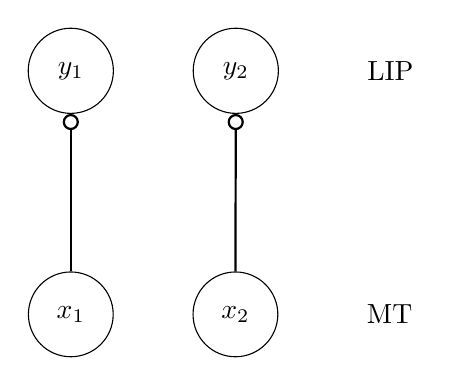
\begin{tikzpicture}
\node[circle,align=center,text width = 0.75cm, draw=black](y1){$y_1$};
\node[circle,align=center,text width = 0.75cm, draw=black,right = 1cm of y1](y2){$y_2$};
\node[right = 1cm of y2](lip){LIP};
\node[circle,align=center,text width = 0.75cm, draw=black,below = 2cm of y1](x1){$x_1$};
\node[circle,align=center,text width = 0.75cm, draw=black,right = 1cm of x1](x2){$x_2$};
\node[right = 1cm of x2](mt){MT};
\draw (x1)edge[thick,-o](y1);
\draw (x2)edge[thick,-o](y2);
\end{tikzpicture}
\end{center}
\caption{The race model. Each direction in MT feeds forward to be
  integrated in LIP; the nodes here might correspond to neurons or to
  collections of neurons, but either way the LIP nodes sum up the
  activity of the different noisy direction signals recorded at MT.\label{fig:race}}
\end{figure}

\subsection*{Feedforward inhibition model}

The feedforward inhibition model is like the race model except the MT
neurons excite their own neuron and inhibit the other, giving one
neuron with rising activity and one with falling \cite{ShadlenNewsome2001a}. This is illustrated
in Fig.~\ref{fig:ffh}. This time we have
\begin{eqnarray}
y_1&=&\int^t [x_1(s)-x_2(s)]ds\cr
y_2&=&\int^t [x_2(s)-x_1(s)]ds
\end{eqnarray}
with the decision made if the denoised signal $y_1$ or $y_2$ exceeds
$Z$, this time we should think of the $y_i$ as starting at some
intermediate value, so they can fall as well as rise. This fits the
data well and is not dissimilar from the drift diffusion model;
$\langle x_1-x_2\rangle$ should depend on how unambiguous the task is,
$Z$ controls the pay-off between speed and accuracy and variations in
the initial values of the $y_i$ reflect the bias.

\begin{figure}
\begin{center}
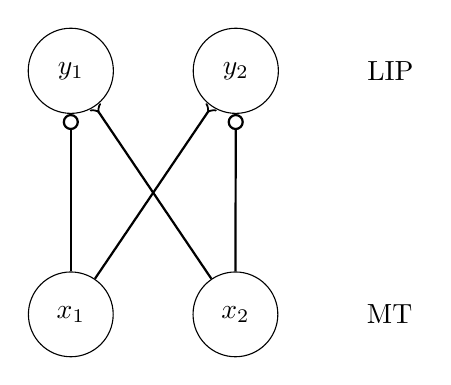
\begin{tikzpicture}
\node[circle,align=center,text width = 0.75cm, draw=black](y1){$y_1$};
\node[circle,align=center,text width = 0.75cm, draw=black,right = 1cm of y1](y2){$y_2$};
\node[right = 1cm of y2](lip){LIP};
\node[circle,align=center,text width = 0.75cm, draw=black,below = 2cm of y1](x1){$x_1$};
\node[circle,align=center,text width = 0.75cm, draw=black,right = 1cm of x1](x2){$x_2$};
\node[right = 1cm of x2](mt){MT};
\draw (x1)edge[thick,-o](y1);
\draw (x2)edge[thick,-o](y2);
\draw (x1)edge[thick,-<](y2);
\draw (x2)edge[thick,-<](y1);
\end{tikzpicture}
\end{center}
\caption{The feedforward inhibition model. Each direction in MT feeds forward to be
  integrated in LIP, adding to some neurons and inhibiting others.\label{fig:ffh}}
\end{figure}

\subsection*{Sequential probability ratio test}

In fact, it is possible to argue that the feedforward inhibition model
implements an optimal strategy for dealing with this problem. To see
this we need to reformulate the problem statistically
\cite{GoldShadlen2001a}. Say $x_i(t)$ is the firing rate of MT neurons
selective for $i$ at time $t$. The goal is to decide whether $x_1$ or
$x_2$ has the highest mean. Now, imagine $x_1$ and $x_2$ are normally
distributed with the same variance and that there are two
possibilities, $x_1$ has mean $\mu_1$ and $x_2$ has mean $\mu_2$, or
visa versa, with $\mu_1>\mu_2$. Thus, one hypothesis, $H_1$, is that
\begin{equation}
x_1\sim \mathcal{N}(\mu_1,\sigma),\quad x_2\sim \mathcal{N}(\mu_2,\sigma)
\end{equation}
and the other, $H_2$, is that
\begin{equation}
x_1\sim \mathcal{N}(\mu_2,\sigma),\quad x_2\sim \mathcal{N}(\mu_1,\sigma)
\end{equation}
The challenge is to decide as quickly as possible which of $x_1$ and
$x_2$ has the higher mean by measuring them.

The optimal solution to this problem is actually known and is provided
by the sequential probability ratio test (SPRT) \cite{Wald1947a}. After each sample the quantity
\begin{equation}
R=\frac{P(\textbf{x}(t_1),\ldots,\textbf{x}(t_n)|H_1)}{P(\textbf{x}(t_1),\ldots,\textbf{x}(t_n)|H_2)}
\end{equation}
where $\textbf{x}(t_i)$ is the value of the $x_i$ at the sample time
$t_i$ and $t_n$ is the most recent sample time. Now, if $R>Z_1$ decide
$H_1$ is true, if $R<Z_2$ decide $H_2$ is, otherwise continue
sampling.

Now, if the sample points are independent
\begin{equation}
P(\textbf{x}(t_1),\ldots,\textbf{x}(t_n)|H_a)=\prod_{i=1}^nP(\textbf{x}(t_i)|H_a)
\end{equation}
for $a=1$ or $a=2$ and, in the usual way, this product is turned into a sum by taking the logarithm:
\begin{equation}
\log{P(\textbf{x}(t_1),\ldots,\textbf{x}(t_n)|H_a)}=\sum_{i=1}^n\log{P(\textbf{x}(t_i)|H_a)}
\end{equation}
In fact, we know 
\begin{equation}
P(\textbf{x}(t_i)|H_1)=\frac{1}{2\pi\sigma^2}e^{-(x_1(t_i)-\mu_1)/2\sigma^2}e^{-(x_2(t_i)-\mu_2)/2\sigma^2}
\end{equation}
and so on, so we can substitute explicitly into the formula for $\log{R}$, in fact, lots of stuff cancels and we get
\begin{equation}
\log{R}=\frac{\mu_1-\mu_2}{\sigma^2}\sum_{i=1}^n[x_1(t_i)-x_2(t_i)]
\end{equation}
This model is clearly implemented by feedforward inhibition. It is
also optimal, it is shown in \cite{WaldWolfowitz1948a} that given
level of error the SPRT arrives quickest at an answer. Thus, if the
parameters are chosen appropriately the race model and feedforward
inhibition model can be chosen to have the same chance of error but
the feedforward inhibitory model will be quicker.
 

\begin{thebibliography}{10}

\bibitem{AshbyEnnisSpiering2007a}
Ashby FG, Ennis JM, Spiering BJ. (2007) A neurobiological theory of automaticity in perceptual categorization. 
\newblock Psychological Review. 114: 632.

\bibitem{RatcliffVanZandtMcKoon1999a}
Ratcliff R, Van Zandt T, McKoon G. (1999) Connectionist and diffusion models of reaction time. 
\newblock Psychological Review. 106: 261.

\bibitem{Ratcliff1978a}
Ratcliff R. (1978) A theory of memory retrieval. 
\newblock Psychological Review. 85: 59.

\bibitem{Ratcliff1979a}
Ratcliff R. (1979) Group reaction time distributions and an analysis of distribution statistics. 
\newblock Psychological Bulletin. 86: 446.

\bibitem{WieckiSoferFrank2013a}
Wiecki TV, Sofer I,  Frank MJ. (2013) HDDM: Hierarchical Bayesian estimation of the Drift-Diffusion Model in Python.
\newblock Frontiers in Neuroinformatics. 7: 14.

\bibitem{RoitmanShadlen2002a}
Roitman JD, Shadlen MN. (2002) Response of neurons in the lateral intraparietal area during a combined visual discrimination reaction time task. 
\newblock The Journal of Neuroscience, 22: 9475--9489.

\bibitem{Vickers1970a}
Vickers D. (1970) Evidence for an accumulator model of psychophysical discrimination. 
\newblock Ergonomics. 13: 37--58.

\bibitem{ShadlenNewsome2001a}
Shadlen MN, Newsome WT. (2001) Neural basis of a perceptual decision in the parietal cortex (area LIP) of the rhesus monkey. 
\newblock Journal of Neurophysiology, 86: 1916--1936.

\bibitem{GoldShadlen2001a}
Gold JI, Shadlen MN. (2001) Neural computations that underlie decisions about sensory stimuli. 
\newblock Trends in Cognitive Sciences, 5: 10--16.

\bibitem{Wald1947a}
Wald A. (1947) Sequential analysis.
\newblock New York: Wiley \& Sons.

\bibitem{WaldWolfowitz1948a}
Wald A, Wolfowitz J (1948). Optimum character of the sequential probability ratio test. 
\newblock The Annals of Mathematical Statistics 19: 326--339.

\end{thebibliography}

\end{document}
